\begin{figure}[h]
\centering
\begin{subfigure}[b]{0.3\textwidth}
    \centering
    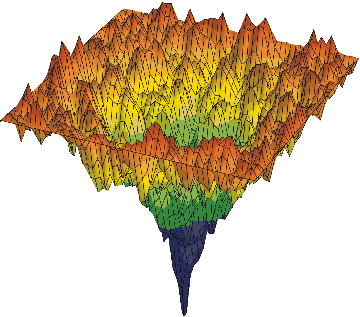
\includegraphics[width=\textwidth]{figures/drysurf.png}
    \label{fig:dry}
    \caption{}
\end{subfigure}%
\hspace{0.1\textwidth}
\begin{subfigure}[b]{0.3\textwidth}
    \centering
    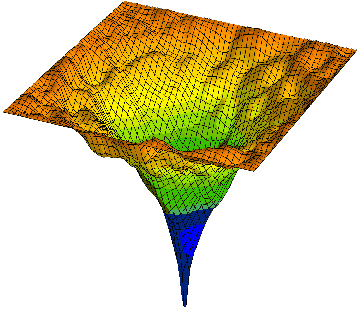
\includegraphics[width=\textwidth]{figures/wetsurf.png}
    \label{fig:wet}
    \caption{}
\end{subfigure}
\caption{
Here energy is represented as a function of the two principal components of the protein conformation, in both cases the approximate funnel shape of the energy surface about the native conformation is very apparent.
(a) shows an energy surface without any solvent effects.
(b) represents a surface with the effect of hydration, though this surface appears smooth relative the dry surface in reality all energy landscapes of larger proteins contain many local minima.
Figure from \protect\cite{waterwebsite} used with authors permission.
}
\label{fig:funnel}
\end{figure}
